%% Presentación Proyecto 6 – Computación Bio-inspirada
%% Máster en Inteligencia Artificial – Universidad de Murcia

%%%%%%%%%%%%%%%%%%%%%%%%%%%%
\documentclass[10pt, envcountsect, presentation, aspectratio=169]{beamer}
%%%%%%%%%%%%%%%%%%%%%%%%%%%%

%%%%%%%%%%%%%%%%%%%%%%%%%%%%
\input plantillaMasterIA.sty
%%%%%%%%%%%%%%%%%%%%%%%%%%%%

\usepackage{booktabs}

%%%%%%%%%%%%%%%%%%%%%%%%%%%%
\title[PenTiDef]{Extensiones de Machine Learning}
\subtitle{PenTiDef}

\author[G. Carmona, V. Saura, F.J. Cortes]
{%
	\sc{Víctor Saura Meseguer}\\
	\\
	\sc{Francisco José Cortes Delgado}\\
	\\
    \sc{Guillermo Carmona Martínez}\\
    \\
}

\institute[UMU]
{
	\textit{Universidad de Murcia}
}

\date{2025/2026}
%%%%%%%%%%%%%%%%%%%%%%%%%%%%

\setbeamerfont{normal text}{size=\normalsize}
\AtBeginDocument{\usebeamerfont{normal text}}

\begin{document}

%%%%%%%%%%%%%%%%%%%%%%%%%%%%%%%%%%
%% PORTADA
%%%%%%%%%%%%%%%%%%%%%%%%%%%%%%%%%%
\begin{frame}[plain]
	\titlepage
\end{frame}

%%%%%%%%%%%%%%%%%%%%%%%%%%%%%%%%%%
%% ÍNDICE
%%%%%%%%%%%%%%%%%%%%%%%%%%%%%%%%%%
\begin{frame}{Índice}{}
	\begin{itemize}
		\item 1. Introducción.
        \item 2. Estado del arte.
        \item 3. Amenazas contempladas.
        \item 4. Estructura y funcionamiento.
        \item 5. Resultados. 
        \item 6. Conclusiones.
	\end{itemize}
\end{frame}

\section{Introducción}
\begin{frame}{1. Introducción}{Contexto}
  \begin{columns}[T]
    \begin{column}{0.5\textwidth}
      \textbf{IDS + Machine Learning}\\[0.3em]
      \begin{itemize}
        \item Detectan intrusiones por patrones de tráfico
        \item Necesitan datos diversos y abundantes
        \item Reentrenamiento continuo ante nuevas amenazas
      \end{itemize}
    \end{column}
    \begin{column}{0.5\textwidth}
      \textbf{El dilema de los datos}\\[0.3em]
      \begin{itemize}
        \item Tráfico real $=$ información sensible
        \item Privacidad y normativa bloquean compartirlo
        \item \textcolor{UMUblue}{\textbf{FL}}: entrenar sin mover los datos
      \end{itemize}
    \end{column}
  \end{columns}
  \vfill
  \begin{block}{}
    \centering ¿Y si el propio FL clásico es el siguiente cuello de botella?
  \end{block}
\end{frame}

\begin{frame}{1. Introducción}{Limitaciones del FL centralizado}
  \begin{center}
  \begin{tikzpicture}[
    client/.style ={draw=UMUblue, rounded corners, minimum width=1.6cm,
                     minimum height=0.6cm, font=\scriptsize},
    server/.style ={draw=UMUblue, fill=UMUblue!20, rounded corners,
                     minimum width=2.6cm, minimum height=0.9cm,
                     font=\small\bfseries, align=center},
    badge/.style  ={draw=red!70!black, fill=yellow!30, rounded corners,
                     font=\tiny\bfseries, align=center, inner sep=2pt}
  ]
    \node[server] (S) at (0,0) {Servidor agregador};
    \node[badge, anchor=south] at ($(S.north)+(0,0.08)$)
      {(1) SPOF + servidor confiable obligatorio};

    % Clientes con tonos distintos para sugerir non-IID
    \node[client, fill=blue!5]  (C1) at (-4, 1.4) {Cliente 1};
    \node[client, fill=blue!18] (C2) at (-4,-1.4) {Cliente 2};
    \node[client, fill=blue!32] (C3) at ( 4, 1.4) {Cliente 3};
    \node[client, fill=blue!45] (C4) at ( 4,-1.4) {Cliente 4};

    \draw[<->, thick, UMUblue] (C1) -- (S);
    \draw[<->, thick, UMUblue] (C2) -- (S);
    \draw[<->, thick, UMUblue] (C3) -- (S);
    \draw[<->, thick, UMUblue] (C4) -- (S);

    \node[font=\tiny, UMUblue] at (-2.4, 0.25) {modelos};

    \node[badge, anchor=north] at (0,-2.0)
      {(2) Distribuciones non-IID heterogéneas};
  \end{tikzpicture}
  \end{center}
  \vspace{-0.4em}
  \begin{itemize}\small
    \item \textbf{(1)} SPOF: si cae el agregador, cae todo el sistema
    \item Servidor central $=$ cuello de botella de comunicación
    \item \textbf{(2)} Heterogeneidad \textbf{non-IID} complica cualquier defensa
  \end{itemize}
\end{frame}

\section{Estado del arte}
\begin{frame}{2. Estado del arte}{Ataques sobre FL}
  \begin{center}
  \begin{tikzpicture}[
    root/.style ={draw=UMUblue, fill=UMUblue!20, rounded corners,
                   font=\small\bfseries, minimum width=3cm,
                   minimum height=0.6cm, align=center},
    cat/.style  ={draw=UMUblue, rounded corners, font=\small\bfseries,
                   minimum width=3.2cm, minimum height=0.6cm, align=center},
    sub/.style  ={font=\scriptsize, align=center}
  ]
    \node[root] (R) at (0,0.4) {Ataques sobre FL};
    \node[cat, fill=blue!8]  (P) at (-3.5,-1.0) {Privacidad};
    \node[cat, fill=red!10]  (V) at ( 3.5,-1.0) {Envenenamiento};

    \node[sub, anchor=north, text width=4.2cm] at (-3.5,-1.5)
      {GAN: reconstruir muestras\\Membership inference};
    \node[sub, anchor=north, text width=4.6cm] at ( 3.5,-1.5)
      {Data poisoning (label flipping)\\Model poisoning (weight scaling)};

    \draw[->, thick, UMUblue]      (R) -- (P);
    \draw[->, thick, red!70!black] (R) -- (V);
  \end{tikzpicture}
  \end{center}
  \vfill
  \begin{itemize}\small
    \item Privacidad: gradientes revelan clases, atributos y muestras
    \item Envenenamiento: \textit{untargeted} (degrada) vs \textit{targeted} (backdoor)
  \end{itemize}
\end{frame}


\begin{frame}{2. Estado del arte}{Defensas existentes y sus límites}
  \begin{columns}[T]
    \begin{column}{0.5\textwidth}
      \textbf{Privacidad}\\[0.2em]
      \begin{itemize}\small
        \item \textbf{HE} (cifrado homomórfico): \textcolor{red!70!black}{coste enorme}
        \item \textbf{SMPC}: alto coste y sincronización
        \item \textbf{DP} diferencial: ligera y escalable
        \item Variantes: CDP / LDP / \textcolor{UMUblue}{\textbf{DDP}}
      \end{itemize}
    \end{column}
    \begin{column}{0.5\textwidth}
      \textbf{Robustez (espacio latente)}\\[0.2em]
      \begin{itemize}\small
        \item \textbf{FLARE}: dataset auxiliar $\rightarrow$ \textcolor{red!70!black}{rompe privacidad}
        \item \textbf{FedCC}: PLR directo $\rightarrow$ \textcolor{red!70!black}{inestable non-IID}
        \item \textbf{Fed-LSAE}: AutoEncoder, pero PLR aún grande
        \item Todos asumen un \textcolor{red!70!black}{servidor central}
      \end{itemize}
    \end{column}
  \end{columns}
\end{frame}

\begin{frame}{2. Estado del arte}{Brecha que motiva PenTiDef}
  \begin{block}{Ningún trabajo previo cubre simultáneamente:}
    \begin{itemize}
      \item \textbf{Descentralización}: sin servidor confiable
      \item \textbf{Privacidad}: sin asumir confianza en el agregador
      \item \textbf{Robustez}: bajo distribuciones non-IID
    \end{itemize}
  \end{block}
  \vfill
  \begin{center}
    \textit{PenTiDef} $=$ \textbf{(Pen)}ultimate \textbf{(T)}rust \\
    pr\textbf{(i)}vacy preserving \textbf{(De)}centralized \textbf{(F)}ederated IDS
  \end{center}
\end{frame}

% --- 1. Modelo de Amenaza (Sección 3) ---
\begin{frame}{3. Amenazas contempladas}{Supuestos y Estrategias de Ataque}
    \begin{block}{3.1 Configuración del Sistema}
        \begin{itemize}
            \item Se asumen 20 colaboradores con una proporción de atacantes del 10\%, 20\% y 40\%.
            \item El entrenamiento dura 10 rondas; los ataques se ejecutan desde la primera.
        \end{itemize}
    \end{block}

    \begin{columns}[t]
        \begin{column}{0.48\textwidth}
            \textbf{Ataques No Dirigidos}
            \begin{itemize}
                \item \textbf{Label-flipping:} Inversión de etiquetas (benigno $\leftrightarrow$ ataque).
                \item \textbf{Weight Scaling:} Escalado de pesos locales mediante un factor $\lambda > 1$.
                \item \textbf{Untargeted-Krum/Med:} Manipulación para evadir algoritmos de agregación robustos.
            \end{itemize}
        \end{column}
        \begin{column}{0.48\textwidth}
            \textbf{Ataques Dirigidos}
            \begin{itemize}
                \item \textbf{Backdoor:} Inyección de un activador (\textit{trigger}) en los datos para causar comportamientos específicos inesperados.
                \item \textbf{GAN poisoning:} Uso de redes generativas para crear datos falsos que distorsionen el modelo global.
            \end{itemize}
        \end{column}
    \end{columns}
\end{frame}

% --- 2. Componentes Arquitectónicos (Sección 4.1.1) ---
\begin{frame}{4.1.1 Componentes de la Arquitectura}{Estructura del Framework PenTiDef}
    \begin{columns}
        \begin{column}{0.5\textwidth}
            \begin{itemize}
                \item \textbf{Blockchain:} Red permisionada que actúa como orquestador descentralizado.
                \item \textbf{Chaincode:} Smart contracts que ejecutan la validación y filtrado.
                \item \textbf{PLR Extractor:} Obtiene las \textit{Penultimate Layer Representations}.
                \item \textbf{AutoEncoder (AE):} Comprime las PLR en \textit{Latent Space Representations} (LSR).
                \item \textbf{KMeans:} Agrupa los modelos según su similitud CKA para aislar atacantes.
            \end{itemize}
        \end{column}
        \begin{column}{0.5\textwidth}
            \begin{figure}
                \centering
                % Reemplaza 'diagrama_arquitectura' por el nombre de tu archivo de imagen
                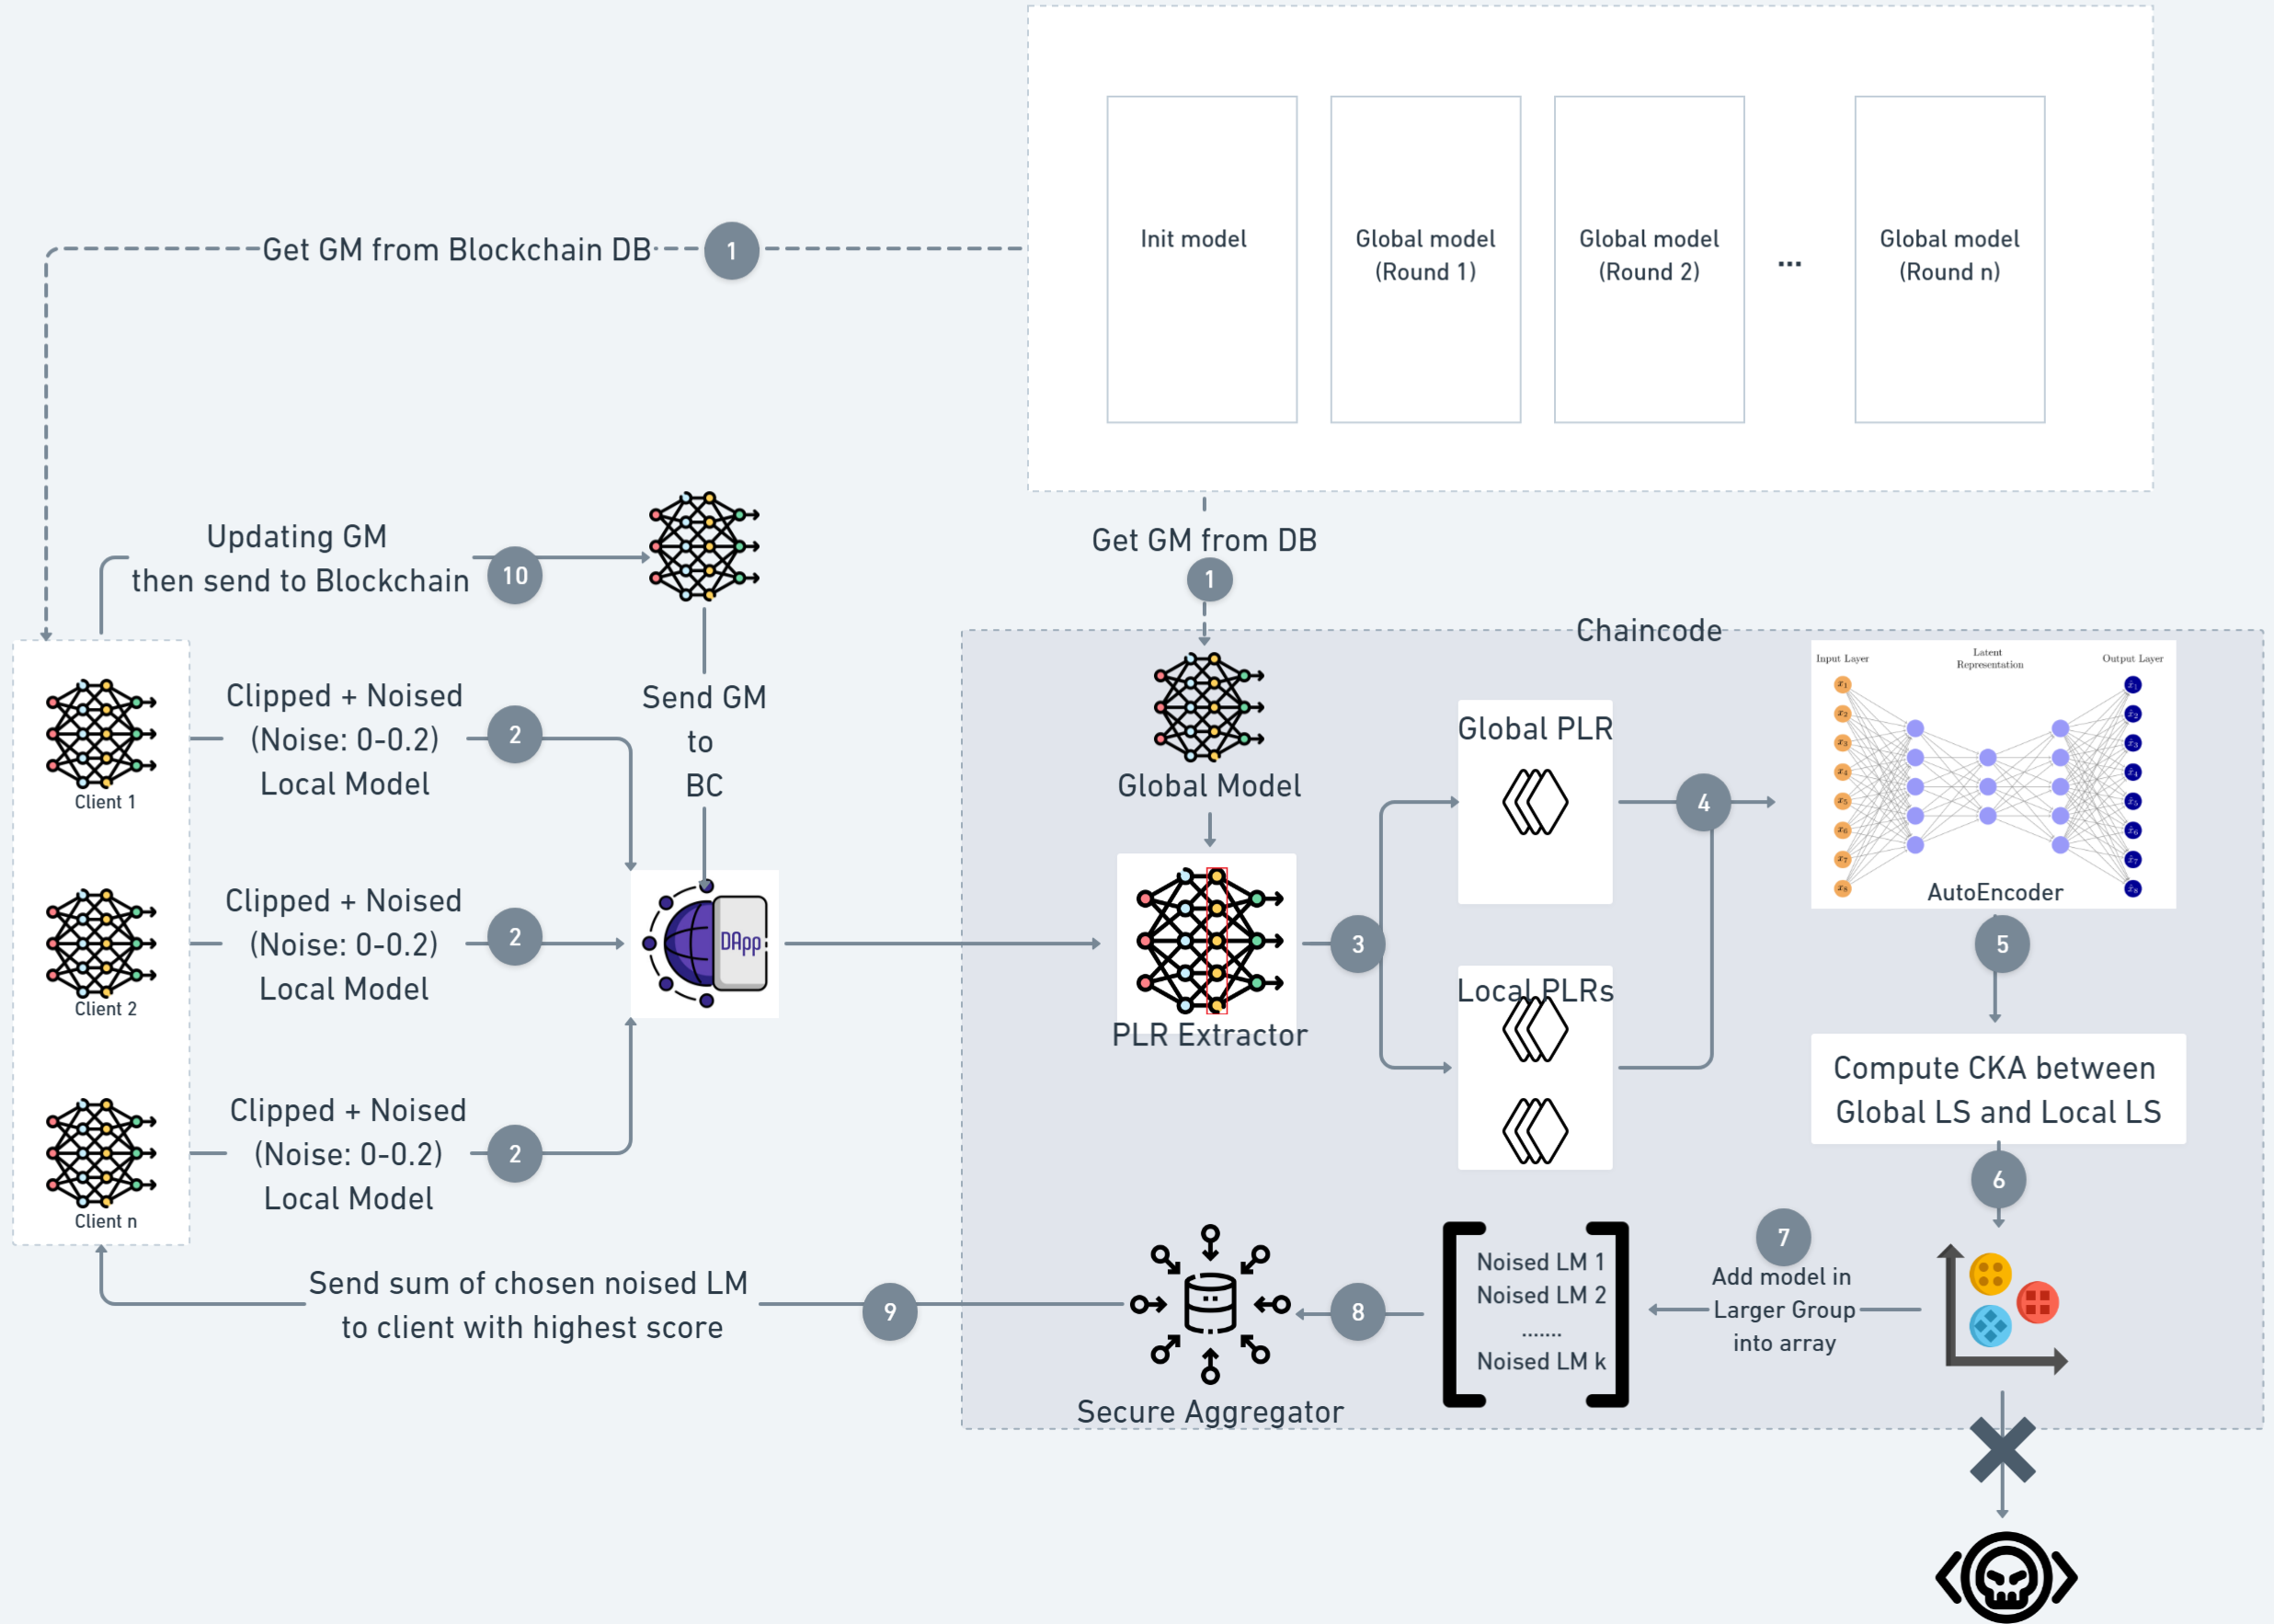
\includegraphics[width=\textwidth]{images/ArquitecturaPentidef.png}
                \caption{Arquitectura PenTiDef}
            \end{figure}
        \end{column}
    \end{columns}
\end{frame}

% --- 3. Principios de Funcionamiento (Sección 4.1.2) ---
\begin{frame}{4.1.2 Principios de Funcionamiento}{Algoritmo y Flujo de Trabajo}
    \begin{enumerate}
        \item \textbf{Recuperación:} Los clientes obtienen el modelo global (GM) de la blockchain.
        \item \textbf{Entrenamiento y Ruido:} Entrenamiento local seguido de perturbación por ruido DDP.
        \item \textbf{Extracción PLR:} Los modelos enviados extraen sus representaciones de la penúltima capa.
        \item \textbf{Reducción LSR:} El AutoEncoder comprime las PLR para mayor estabilidad ante datos no-IID.
        \item \textbf{Similitud CKA:} Se calcula la similitud entre el GM y los modelos locales.
        \item \textbf{Clustering:} KMeans divide los modelos en grupos mayoritarios (benignos) y minoritarios (atacantes).
        \item \textbf{Agregación:} Solo los modelos benignos se combinan mediante el \textit{Secure Aggregator}.
        \item \textbf{Actualización:} El cliente más confiable propaga el nuevo GM a la red.
    \end{enumerate}
\end{frame}

% --- 4. DDP con Nivel de Ruido Aleatorio (Sección 4.2) ---
\begin{frame}{4.2 DDP con Nivel de Ruido Aleatorio}{Privacidad Diferencial Distribuida}
    \begin{itemize}
        \item \textbf{Mecanismo Gaussiano:} Se define como $\mathcal{M}(w) = w + \mathcal{N}(0, \sigma^2)$ para proteger los pesos locales.
    \end{itemize}
    \begin{exampleblock}{Aleatoriedad de $\sigma$}
        Para evitar que los adversarios infieran patrones de ruido, PenTiDef selecciona $\sigma$ aleatoriamente del intervalo $[0, 0.2]$ en cada ronda.
    \end{exampleblock}
    \begin{itemize}
        \item \textbf{Beneficio:} Previene ataques de reconstrucción.
        \item \textbf{Transparencia:} Los niveles de ruido se registran en la blockchain para auditoría.
    \end{itemize}
\end{frame}

% --- 5. Integración de Blockchain (Sección 4.3) ---
\begin{frame}{4.3 Integración de Blockchain}{Coordinación en Federated Learning}
    \begin{itemize}
        \item \textbf{Hyperledger Fabric:} Red permisionada (ni pública ni anónima) de 3 organizaciones y 6 nodos pares para mayor tolerancia a fallos.
        \item \textbf{Gestión de Identidad:} Uso de certificados digitales $(ID_i, SK_i)$ para firmar transacciones y asegurar autenticidad.
        \item \textbf{Almacenamiento Híbrido:}
        \begin{itemize}
            \item \textbf{On-chain:} Hashes de los modelos $h(w_i^t)$ y metadatos de auditoría.
            \item \textbf{Off-chain:} Parámetros del modelo almacenados en \textbf{IPFS} para evitar cuellos de botella.
        \end{itemize}
        \item \textbf{Transparencia:} Garantiza que solo actualizaciones verificadas entren en el estado de aprendizaje global.
    \end{itemize}
\end{frame}

% =====================================================================
% Parte de Francisco José Cortés Delgado
% Cubre secciones 5 (Research Questions), 6 (Implementation & Metrics),
% 7 (Experimental Results), 8 (Discussion) y 9 (Conclusion) del paper.
% =====================================================================

\section{Resultados}

% --- 1. Preguntas de investigación (Sección 5.1) ---
\begin{frame}{5. Resultados}{Preguntas de investigación}
  \begin{columns}[T]
    \begin{column}{0.49\textwidth}
      \textbf{Efectividad del framework}\\[0.3em]
      \begin{itemize}\small
        \item \textbf{RQ1:} ¿Cómo afecta DDP al rendimiento del modelo?
        \item \textbf{RQ3:} ¿PenTiDef frente a FLARE y FedCC?
        \item \textbf{RQ4:} ¿Detecta ataques \textit{targeted} y \textit{untargeted}?
      \end{itemize}
    \end{column}
    \begin{column}{0.49\textwidth}
      \textbf{Robustez y escalabilidad}\\[0.3em]
      \begin{itemize}\small
        \item \textbf{RQ2:} ¿Comportamiento bajo IID vs non-IID?
        \item \textbf{RQ5:} ¿Coste computacional y tiempo de entrenamiento?
        \item \textbf{RQ6:} ¿Estabilidad cambiando la arquitectura DL?
        \item \textbf{RQ7:} ¿Rendimiento de la capa blockchain?
      \end{itemize}
    \end{column}
  \end{columns}
  \vfill
  \begin{block}{}
    \centering Siete preguntas $\Rightarrow$ cuatro escenarios experimentales.
  \end{block}
\end{frame}

% --- 2. Escenarios experimentales (Sección 5.2) ---
\begin{frame}{5. Resultados}{Escenarios experimentales}
  \begin{center}
  \small
  \begin{tabular}{@{}clll@{}}
    \toprule
    \textbf{\#} & \textbf{Escenario} & \textbf{Foco} & \textbf{RQs} \\
    \midrule
    1 & Impacto de DDP           & PenTiDef con y sin ruido DDP            & RQ1 \\
    2 & Comparativa de defensas  & vs.\ FLARE y FedCC, IID y non-IID       & RQ2--RQ5 \\
    3 & Cross-architecture       & CNN vs.\ SqueezeNet                     & RQ5, RQ6 \\
    4 & Capa blockchain          & Latencia y \textit{throughput} (Fabric) & RQ7 \\
    \bottomrule
  \end{tabular}
  \end{center}
  \vfill
  \begin{itemize}\small
    \item Cada escenario responde a una o varias RQs.
    \item Combinan \textbf{detección}, \textbf{coste} y \textbf{coordinación}.
  \end{itemize}
\end{frame}

% --- 3. Configuración (Sección 6.1, 6.3, 6.4) ---
\begin{frame}{5. Resultados}{Configuración experimental}
  \begin{columns}[T]
    \begin{column}{0.5\textwidth}
      \textbf{Entorno}\\[0.2em]
      \begin{itemize}\small
        \item AMD Ryzen 7 6800HS + 16 GB RAM
        \item Hyperledger Fabric (3 orgs, 6 nodos)
        \item IPFS para \textit{off-chain storage}
        \item 20 clientes; atacantes: 10 / 20 / 40\%
        \item 10 rondas FL, ataques desde la 1ª
      \end{itemize}
    \end{column}
    \begin{column}{0.5\textwidth}
      \textbf{Modelo IDS}\\[0.2em]
      \begin{itemize}\small
        \item CNN 1D (11 capas ocultas), Adam + ReLU
        \item Batch 1024, 5 épocas locales
        \item SqueezeNet como \textit{backbone} alternativo
      \end{itemize}
    \end{column}
  \end{columns}
  \vfill
  \textbf{Datasets:}
  \begin{itemize}\small
    \item \textbf{CIC-IDS2018}: 71 \textit{features}, 42.6\% benigno / 57.4\% ataque.
    \item \textbf{Edge-IIoTSet}: 95 \textit{features}, 71.4\% benigno / 28.6\% ataque.
    \item 70\% \textit{train} / 30\% \textit{test}; particiones IID y non-IID.
  \end{itemize}
\end{frame}

% --- 4. Métricas (Sección 6.5) ---
\begin{frame}{5. Resultados}{Métricas de evaluación}
  \begin{columns}[T]
    \begin{column}{0.55\textwidth}
      \textbf{Clasificación binaria}\\[0.3em]
      \begin{itemize}\small
        \item \textbf{Accuracy}: clasificaciones correctas totales.
        \item \textbf{Precision}: fiabilidad de la detección positiva.
        \item \textbf{Recall}: cobertura de ataques reales.
        \item \textbf{F1-Score}: media armónica (balancea \textit{precision} y \textit{recall}).
      \end{itemize}
    \end{column}
    \begin{column}{0.45\textwidth}
      \textbf{Filtrado de clientes}\\[0.3em]
      \begin{itemize}\small
        \item \textbf{CKA Score}: similitud entre espacios latentes.
        \begin{itemize}\scriptsize
          \item CKA alto $\Rightarrow$ benigno.
          \item CKA bajo $\Rightarrow$ candidato a envenenamiento.
        \end{itemize}
        \item \textbf{Tiempo medio} como \textit{proxy} de coste.
        \item \textbf{Latencia / TPS} para la capa blockchain.
      \end{itemize}
    \end{column}
  \end{columns}
\end{frame}

% --- 5. Resultado 1: Impacto de DDP ---
\begin{frame}{5.1 Resultado 1}{Impacto de DDP sobre el rendimiento (RQ1)}
  \begin{columns}[T]
    \begin{column}{0.5\textwidth}
      \begin{itemize}\small
        \item \textbf{Sin DDP:} convergencia rápida, $\sim$0.98 desde la ronda 3.
        \item \textbf{Con DDP} ($\sigma \in [0, 0.2]$): arranque más lento por el ruido, estabiliza hacia la ronda 10.
        \item Diferencia final en Accuracy, Precision, Recall y F1: $\approx$ \textbf{0.01}.
      \end{itemize}
    \end{column}
    \begin{column}{0.5\textwidth}
      \begin{tikzpicture}[scale=0.75]
        % Rejilla
        \foreach \y/\lbl in {1/0.7, 2/0.8, 3/0.9, 4/1.0} {
           \draw[gray!30] (0.05,\y) -- (5.2,\y);
           \node[font=\tiny, gray!70, anchor=east] at (-0.05,\y) {\lbl};
        }
        % Ejes sin flechas
        \draw[thick] (0,0) -- (5.2,0);
        \draw[thick] (0,0) -- (0,4.4);
        % Curvas
        \draw[UMUblue, thick]
          plot[smooth] coordinates {(0.3,1.8) (1,3.0) (2,3.6) (3,3.8) (4,3.9) (5,3.95)};
        \draw[red!70!black, thick, dashed]
          plot[smooth] coordinates {(0.3,0.5) (1,1.5) (2,2.6) (3,3.3) (4,3.7) (5,3.85)};
        % Etiquetas de curvas
        \node[UMUblue, font=\scriptsize, anchor=west] at (3.3, 4.2) {non-DDP};
        \node[red!70!black, font=\scriptsize, anchor=west] at (3.3, 2.9) {DDP};
        % Etiquetas de ejes
        \node[font=\scriptsize, anchor=north] at (2.6,-0.2) {ronda};
        \node[font=\scriptsize, rotate=90, anchor=south] at (-0.8,2.2) {métrica};
      \end{tikzpicture}
    \end{column}
  \end{columns}
  \vfill
  \begin{exampleblock}{Conclusión}
    \centering DDP añade \textbf{privacidad por diseño} con un coste prácticamente despreciable en utilidad.
  \end{exampleblock}
\end{frame}

% --- 6. Resultado 2a: Ataques no dirigidos IID ---
\begin{frame}{5.2 Resultado 2}{Ataques no dirigidos (IID, F1-Score)}
  \begin{center}
  \scriptsize
  \begin{tabular}{@{}llccc|ccc@{}}
    \toprule
    & & \multicolumn{3}{c|}{\textbf{Adversarios 20\%}} & \multicolumn{3}{c}{\textbf{Adversarios 40\%}} \\
    \textbf{Dataset} & \textbf{Ataque} & Flare & FedCC & \textbf{PenTiDef} & Flare & FedCC & \textbf{PenTiDef} \\
    \midrule
    \multirow{4}{*}{CIC-IDS2018}
      & Label-flipping & 0.93 & 0.95 & \textbf{0.96} & 0.92 & 0.95 & \textbf{0.96} \\
      & Weight-Scaling & \textbf{0.97} & 0.95 & 0.96 & 0.92 & 0.95 & \textbf{0.96} \\
      & Un-Krum        & 0.95 & 0.96 & \textbf{0.97} & \textbf{0.96} & 0.88 & 0.93 \\
      & Un-Med         & 0.95 & 0.93 & \textbf{0.98} & 0.91 & 0.92 & \textbf{0.97} \\
    \midrule
    \multirow{4}{*}{Edge-IIoTSet}
      & Label-flipping & 0.96 & 0.96 & \textbf{0.97} & 0.88 & 0.88 & \textbf{0.92} \\
      & Weight-Scaling & 0.95 & \textbf{0.97} & 0.95 & 0.91 & 0.88 & \textbf{0.95} \\
      & Un-Krum        & \textbf{0.98} & 0.91 & 0.96 & 0.91 & 0.87 & \textbf{0.93} \\
      & Un-Med         & 0.88 & 0.93 & \textbf{0.99} & 0.88 & 0.88 & \textbf{0.95} \\
    \bottomrule
  \end{tabular}
  \end{center}
  \vfill
  \begin{itemize}\small
    \item PenTiDef gana o empata en \textbf{la mayoría} de configuraciones.
    \item A mayor \% de atacantes, mayor ventaja $\Rightarrow$ las defensas rivales se degradan más rápido.
  \end{itemize}
\end{frame}

% --- 7. Resultado 2b: non-IID y CKA ---
\begin{frame}{5.2 Resultado 2}{Discriminación benigno / malicioso (CKA, non-IID)}
  \begin{columns}[T]
    \begin{column}{0.48\textwidth}
      \resizebox{\linewidth}{!}{%
      \begin{tikzpicture}
        % Rejilla horizontal (y = CKA * 6)
        \foreach \y/\lbl in {1.2/0.2, 2.4/0.4, 3.6/0.6, 4.8/0.8, 6.0/1.0} {
           \draw[gray!20] (0.05,\y) -- (14.5,\y);
           \node[font=\scriptsize, gray!70, anchor=east] at (-0.05,\y) {\lbl};
        }
        % PenTiDef benignos (1-12): UMUblue
        \foreach \x/\h in {1/5.10, 2/5.10, 3/5.22, 4/5.16, 5/5.22, 6/4.68, 7/4.92, 8/5.04, 9/4.98, 10/5.22, 11/5.04, 12/5.10} {
          \fill[UMUblue] (\x*0.7-0.32, 0) rectangle (\x*0.7-0.02, \h);
        }
        % PenTiDef atacantes (13-20): rojo (bajada notable)
        \foreach \x/\h in {13/2.88, 14/3.12, 15/3.06, 16/2.88, 17/2.22, 18/2.76, 19/2.88, 20/3.00} {
          \fill[red!65!black] (\x*0.7-0.32, 0) rectangle (\x*0.7-0.02, \h);
        }
        % FedCC todos: apenas baja en atacantes
        \foreach \x/\h in {1/4.98, 2/5.16, 3/5.04, 4/5.22, 5/4.98, 6/4.62, 7/4.74, 8/4.92, 9/4.92, 10/4.80, 11/4.98, 12/5.04, 13/4.62, 14/4.50, 15/4.56, 16/4.68, 17/4.56, 18/4.50, 19/4.56, 20/4.56} {
          \draw[gray!80, fill=gray!25, thick] (\x*0.7+0.02, 0) rectangle (\x*0.7+0.32, \h);
        }
        % Ejes
        \draw[thick] (0,0) -- (14.5,0);
        \draw[thick] (0,0) -- (0,6.5);
        % Separador
        \draw[dashed, gray!70] (8.73, 0) -- (8.73, 6.3);
        % Etiquetas de grupos
        \node[font=\scriptsize, UMUblue, anchor=south] at (4.5, 6.3) {benignos};
        \node[font=\scriptsize, red!70!black, anchor=south] at (11.5, 6.3) {atacantes};
        % Etiquetas de ejes
        \node[font=\scriptsize, anchor=north] at (7.0,-0.5) {clientes 1--20};
        \node[font=\scriptsize, rotate=90, anchor=south] at (-1.2,3) {CKA};
        % Leyenda
        \fill[UMUblue] (1.4,-1.6) rectangle (1.8,-1.25);
        \fill[red!65!black] (4.5,-1.6) rectangle (4.9,-1.25);
        \draw[gray!80, fill=gray!25, thick] (7.9,-1.6) rectangle (8.3,-1.25);
        \node[font=\scriptsize, anchor=west] at (1.9,-1.42) {PenTiDef (benigno)};
        \node[font=\scriptsize, anchor=west] at (5.0,-1.42) {PenTiDef (atacante)};
        \node[font=\scriptsize, anchor=west] at (8.4,-1.42) {FedCC};
      \end{tikzpicture}}
    \end{column}
    \begin{column}{0.52\textwidth}
      \begin{itemize}\small
        \item \textbf{PenTiDef}: CKA $\approx$ 0.85 (benignos) $\to$ $\approx$ 0.45 (atacantes).
        \item \textbf{FedCC}: $\approx$ 0.80 en ambos grupos $\Rightarrow$ no discrimina.
        \item El AutoEncoder + LSR hace la señal \textbf{estable} en non-IID.
      \end{itemize}
      \vfill
      \begin{exampleblock}{¿Por qué PenTiDef discrimina mejor?}
        \scriptsize
        \textbf{FedCC:}\ \ \texttt{PLR $\to$ CKA $\to$ clustering}\\[0.2em]
        \textbf{PenTiDef:}\ \ \texttt{PLR $\to$ AE $\to$ \textcolor{UMUblue}{LSR} $\to$ CKA $\to$ clustering}\\[0.3em]
        El paso \textbf{LSR} limpia ruido, estabiliza representaciones y mejora la separación.
      \end{exampleblock}
    \end{column}
  \end{columns}
\end{frame}

% --- 7b. Resultado 2: Peor caso (40% adversarios, targeted + non-IID) ---
\begin{frame}{5.2 Resultado 2}{Peor caso: 40\% adversarios (F1-Score)}
  \begin{center}
  \small
  \begin{tabular}{@{}lllccc@{}}
    \toprule
    \textbf{Datos} & \textbf{Ataque} & \textbf{Dataset} & \textbf{Flare} & \textbf{FedCC} & \textbf{PenTiDef} \\
    \midrule
    \multirow{4}{*}{IID}
      & GAN-SL  & CIC-IDS2018  & 0.90 & 0.93 & \textbf{0.94} \\
      & GAN-ML  & CIC-IDS2018  & 0.93 & 0.96 & \textbf{0.97} \\
      & GAN-Con & Edge-IIoTSet & 0.93 & 0.92 & \textbf{0.94} \\
      & Backdoor & Edge-IIoTSet & 0.94 & 0.94 & \textbf{0.95} \\
    \midrule
    \multirow{4}{*}{non-IID}
      & Un-Med  & CIC-IDS2018  & 0.87 & 0.88 & \textbf{0.95} \\
      & Un-Krum & CIC-IDS2018  & \textbf{0.92} & 0.84 & 0.89 \\
      & Label-flipping & Edge-IIoTSet & 0.84 & 0.85 & \textbf{0.88} \\
      & Un-Med  & Edge-IIoTSet & 0.84 & 0.84 & \textbf{0.91} \\
    \bottomrule
  \end{tabular}
  \end{center}
  \vfill
  \begin{itemize}\small
    \item Con \textbf{4 de cada 10 clientes maliciosos}, PenTiDef mantiene F1 $\geq$ 0.88 en casi todos los casos.
    \item La caída típica de FLARE/FedCC al pasar a non-IID es de $\sim$0.05--0.10; PenTiDef resiste.
  \end{itemize}
\end{frame}

% --- 8. Resultado 2c: Eficiencia ---
\begin{frame}{5.2 Resultado 2}{Eficiencia: tiempo de entrenamiento}
  \begin{columns}[T]
    \begin{column}{0.5\textwidth}
      \centering
      \small
      \begin{tabular}{@{}llc@{}}
        \toprule
        \textbf{Dataset} & \textbf{Modelo} & \textbf{Tiempo} \\
        \midrule
        \multirow{3}{*}{CIC-IDS2018}
          & FLARE             & 3\,907 s ($\sim$1h 06m) \\
          & FedCC             & 2\,460 s ($\sim$41m) \\
          & \textbf{PenTiDef} & \textbf{1\,988 s ($\sim$33m)} \\
        \midrule
        \multirow{3}{*}{Edge-IIoTSet}
          & FLARE             & 4\,395 s ($\sim$1h 15m) \\
          & FedCC             & 2\,825 s ($\sim$47m) \\
          & \textbf{PenTiDef} & \textbf{1\,869 s ($\sim$31m)} \\
        \bottomrule
      \end{tabular}
    \end{column}
    \begin{column}{0.48\textwidth}
      \textbf{¿Por qué es más rápido?}\\[0.3em]
      \begin{itemize}\small
        \item FLARE requiere un \textit{dataset auxiliar} para comparar PLR.
        \item FedCC compara PLR crudas $\Rightarrow$ vector de gran dimensión.
        \item PenTiDef comprime PLR $\to$ \textbf{LSR} (AutoEncoder) antes de CKA.
      \end{itemize}
      \vfill
      \begin{exampleblock}{}
        \centering $\sim$2$\times$ más rápido que FLARE \\ y sin comprometer detección.
      \end{exampleblock}
    \end{column}
  \end{columns}
\end{frame}

% --- 9. Resultado 3: Cross-architecture ---
\begin{frame}{5.3 Resultado 3}{Robustez entre arquitecturas (RQ5, RQ6)}
  \begin{columns}[T]
    \begin{column}{0.5\textwidth}
      \textbf{Mismo framework, distinto \textit{backbone}}\\[0.3em]
      \begin{itemize}\small
        \item CNN $\leftrightarrow$ SqueezeNet sin rediseñar el filtrado.
        \item Los 4 ataques evaluados, IID y non-IID.
      \end{itemize}
      \vfill
      \textbf{Hallazgos}
      \begin{itemize}\small
        \item CNN $\gtrsim$ SqueezeNet en la mayoría de escenarios.
        \item Ambos mantienen F1 $\geq$ 0.89 con 40\% de atacantes.
        \item La defensa opera sobre la \textbf{penúltima capa}: es \textit{model-agnostic}.
      \end{itemize}
    \end{column}
    \begin{column}{0.5\textwidth}
      \centering
      \scriptsize
      \begin{tabular}{@{}llcc@{}}
        \toprule
        \textbf{Dataset} & \textbf{Ataque} & \textbf{CNN} & \textbf{SqueezeNet} \\
        \midrule
        \multicolumn{4}{c}{\textit{IID · 40\% adversarios}} \\
        \midrule
        CIC-IDS2018  & Label-flipping & 0.94 & \textbf{0.96} \\
        CIC-IDS2018  & Weight-Scaling & 0.96 & \textbf{0.97} \\
        Edge-IIoTSet & Un-Krum        & 0.89 & \textbf{0.90} \\
        \midrule
        \multicolumn{4}{c}{\textit{non-IID · 40\% adversarios}} \\
        \midrule
        CIC-IDS2018  & Label-flipping & 0.93 & \textbf{0.95} \\
        Edge-IIoTSet & Backdoor       & \textbf{0.95} & \textbf{0.95} \\
        \bottomrule
      \end{tabular}
    \end{column}
  \end{columns}
\end{frame}

% --- 10. Resultado 4: Blockchain ---
\begin{frame}{5.4 Resultado 4}{Capa blockchain bajo carga (RQ7)}
  \begin{center}
  \small
  \begin{tabular}{@{}lccc@{}}
    \toprule
    \textbf{Operación} & \textbf{Rate env.} & \textbf{Lat. media} & \textbf{Throughput} \\
    \midrule
    CreateModel              & 5 TPS  & 0.21 s & 28.0 TPS  \\
    CreateModel              & 20 TPS & 0.12 s & 84.5 TPS  \\
    QueryAllModels           & 20 TPS & 0.17 s & 82.1 TPS  \\
    QueryByModelIndex        & 20 TPS & 0.09 s & 177.5 TPS \\
    QueryByBenignClientID    & 20 TPS & 0.31 s & 47.4 TPS  \\
    \bottomrule
  \end{tabular}
  \end{center}
  \vfill
  \begin{itemize}\small
    \item \textbf{0 transacciones fallidas} en 5\,000 y 10\,000 pruebas.
    \item Latencia media $<$ 0.35 s incluso con 10\,000 transacciones.
    \item Hyperledger Fabric soporta la coordinación \textbf{sin cuello de botella}.
  \end{itemize}
\end{frame}

% =====================================================================
\section{Conclusiones}

% --- 11. Discusión ---
\begin{frame}{6. Conclusiones}{Discusión: logros y limitaciones}
  \begin{columns}[T]
    \begin{column}{0.5\textwidth}
      \textbf{\textcolor{UMUblue}{Logros}}\\[0.3em]
      \begin{itemize}\small
        \item Defensa robusta frente a ataques \textit{targeted} y \textit{untargeted}.
        \item Estable bajo non-IID y hasta un \textbf{40\%} de atacantes.
        \item Sin dataset auxiliar ni conocimiento previo de adversarios.
        \item Coordinación \textbf{sin servidor central} vía blockchain.
        \item Menor tiempo de entrenamiento que FLARE y FedCC.
      \end{itemize}
    \end{column}
    \begin{column}{0.5\textwidth}
      \textbf{\textcolor{red!70!black}{Limitaciones}}\\[0.3em]
      \begin{itemize}\small
        \item Sólo clasificación \textbf{binaria} (benigno / ataque).
        \item No evaluado frente a adversarios adaptativos avanzados (\textit{model inversion}, \textit{backdoors} semánticos).
        \item Ruido DDP aleatorio $\to$ posible vector \textit{free-rider}.
        \item Coste de la blockchain no analizado a gran escala.
      \end{itemize}
    \end{column}
  \end{columns}
\end{frame}

% --- 12. Conclusión y trabajo futuro ---
\begin{frame}{6. Conclusiones}{Conclusión y trabajo futuro}
  \begin{block}{Contribución}
    PenTiDef integra \textbf{DDP}, \textbf{LSR + CKA} y \textbf{blockchain} en un framework único de IDS federado descentralizado, superando a FLARE y FedCC en precisión, robustez y eficiencia.
  \end{block}
  \vfill
  \begin{columns}[T]
    \begin{column}{0.5\textwidth}
      \textbf{Trabajo futuro}
      \begin{itemize}\small
        \item Clasificación \textbf{multiclase} de ataques.
        \item Ajuste \textbf{adaptativo} de $\sigma$ en DDP.
        \item Detectores contra \textit{free-riders} y GAN avanzadas.
        \item Explicabilidad (XAI) del filtrado.
      \end{itemize}
    \end{column}
    \begin{column}{0.5\textwidth}
      \textbf{Aplicabilidad}
      \begin{itemize}\small
        \item IoMT y salud conectada.
        \item Edge computing.
        \item Infraestructuras críticas distribuidas.
      \end{itemize}
      \vspace{0.3em}
      \textit{Donde privacidad + descentralización + tiempo real son obligatorias.}
    \end{column}
  \end{columns}
\end{frame}

% --- 13. Cierre ---
\begin{frame}[plain]
  \begin{center}
    \vspace{1.2cm}
    {\Huge \color{UMUblue} \textbf{¿Preguntas?}}\\[1.2cm]
    \textit{PenTiDef} $=$ \textbf{Pen}ultimate \textbf{T}rust \\
    pr\textbf{i}vacy preserving \textbf{De}centralized \textbf{F}ederated IDS \\[1.2cm]
    \small
    Víctor Saura Meseguer · Francisco José Cortés Delgado · Guillermo Carmona Martínez \\[0.4cm]
    Máster en Inteligencia Artificial — Universidad de Murcia
  \end{center}
\end{frame}


\end{document}
